% Created 2026-04-23 Thu 12:08
% Intended LaTeX compiler: lualatex
\DocumentMetadata{lang = en-US,pdfversion = 2.0,pdfstandard = ua-2,tagging = on,tagging-setup = {math/setup=mathml-SE},}
\documentclass[11pt]{article}
\usepackage{amsmath}
\usepackage{fontspec}
\usepackage{graphicx}
\usepackage{longtable}
\usepackage{wrapfig}
\usepackage{rotating}
\usepackage[normalem]{ulem}
\usepackage{capt-of}
\usepackage{hyperref}
\usepackage[margin=1in]{geometry}
\usepackage{fontspec}
\usepackage{verbatim, multicol, tabularx,}
\usepackage{amsmath, amsthm, amssymb, stmaryrd, latexsym, bm, listings, qtree}
\usepackage{framed}
\usepackage{xcolor,colortbl}
\usepackage{media9}
\usepackage[export]{adjustbox}
\usepackage{algorithm}
\usepackage[noend]{algpseudocode}
\usepackage{tikz,pgfplots}
\usetikzlibrary{shapes.geometric}
\let\oldquote=\quote
\let\endoldquote=\endquote
\colorlet{shadecolor}{cyan!15}
\renewenvironment{quote}{\begin{shaded*}\begin{oldquote}}{\end{oldquote}\end{shaded*}}
% From https://tex.stackexchange.com/questions/7032/good-way-to-make-textcircled-numbers
\newcommand*\circled[1]{\tikz[baseline=(char.base)]{\node[shape=circle,draw,inner sep=2pt] (char) {#1};}}
\DeclareMathOperator*{\argmin}{arg\!min}
\DeclareMathOperator*{\argmax}{arg\!max}
\lstset{frame=tb, aboveskip=1mm, belowskip=0mm, showstringspaces=false, columns=flexible, basicstyle={\scriptsize\ttfamily}, numbers=left, frame=single, breaklines=true, breakatwhitespace=true}
\hypersetup{colorlinks=true,urlcolor=blue}
\usepackage{tagpdf}
\tagpdfsetup{activate-all}
\tagpdfsetup{math/alt/use}
\usepackage{polyglossia}
\setdefaultlanguage[variant=en-US]{english}
\author{Christopher Simpkins}
\date{Kennesaw State University}
\title{Artificial Intelligence\\\medskip
\large Local Search}
\hypersetup{
 pdfauthor={Christopher Simpkins},
 pdftitle={Artificial Intelligence},
 pdfkeywords={},
 pdfsubject={Artificial Intelligence Local Search},
 pdfcreator={Emacs 30.2 (Org mode 9.7.11)}, 
 pdflang={English}}
\begin{document}

\maketitle
\section{Local Search}
\label{sec:org5e519e7}

If you don't care about the path to a goal state, you can use \textbf{local search}.

\begin{itemize}
\item Search neighbors of current state, moving to best neighbor.
\item Track only current state.
\item Uses very little memory.
\item Can find reasonable solutions in large or infinite state spaces.
\item Often used for \textbf{optmization} problems -- finding states that maximize or minimize an \textbf{objective function}.
\end{itemize}
\section{State Space Landscape}
\label{sec:org8e234fb}


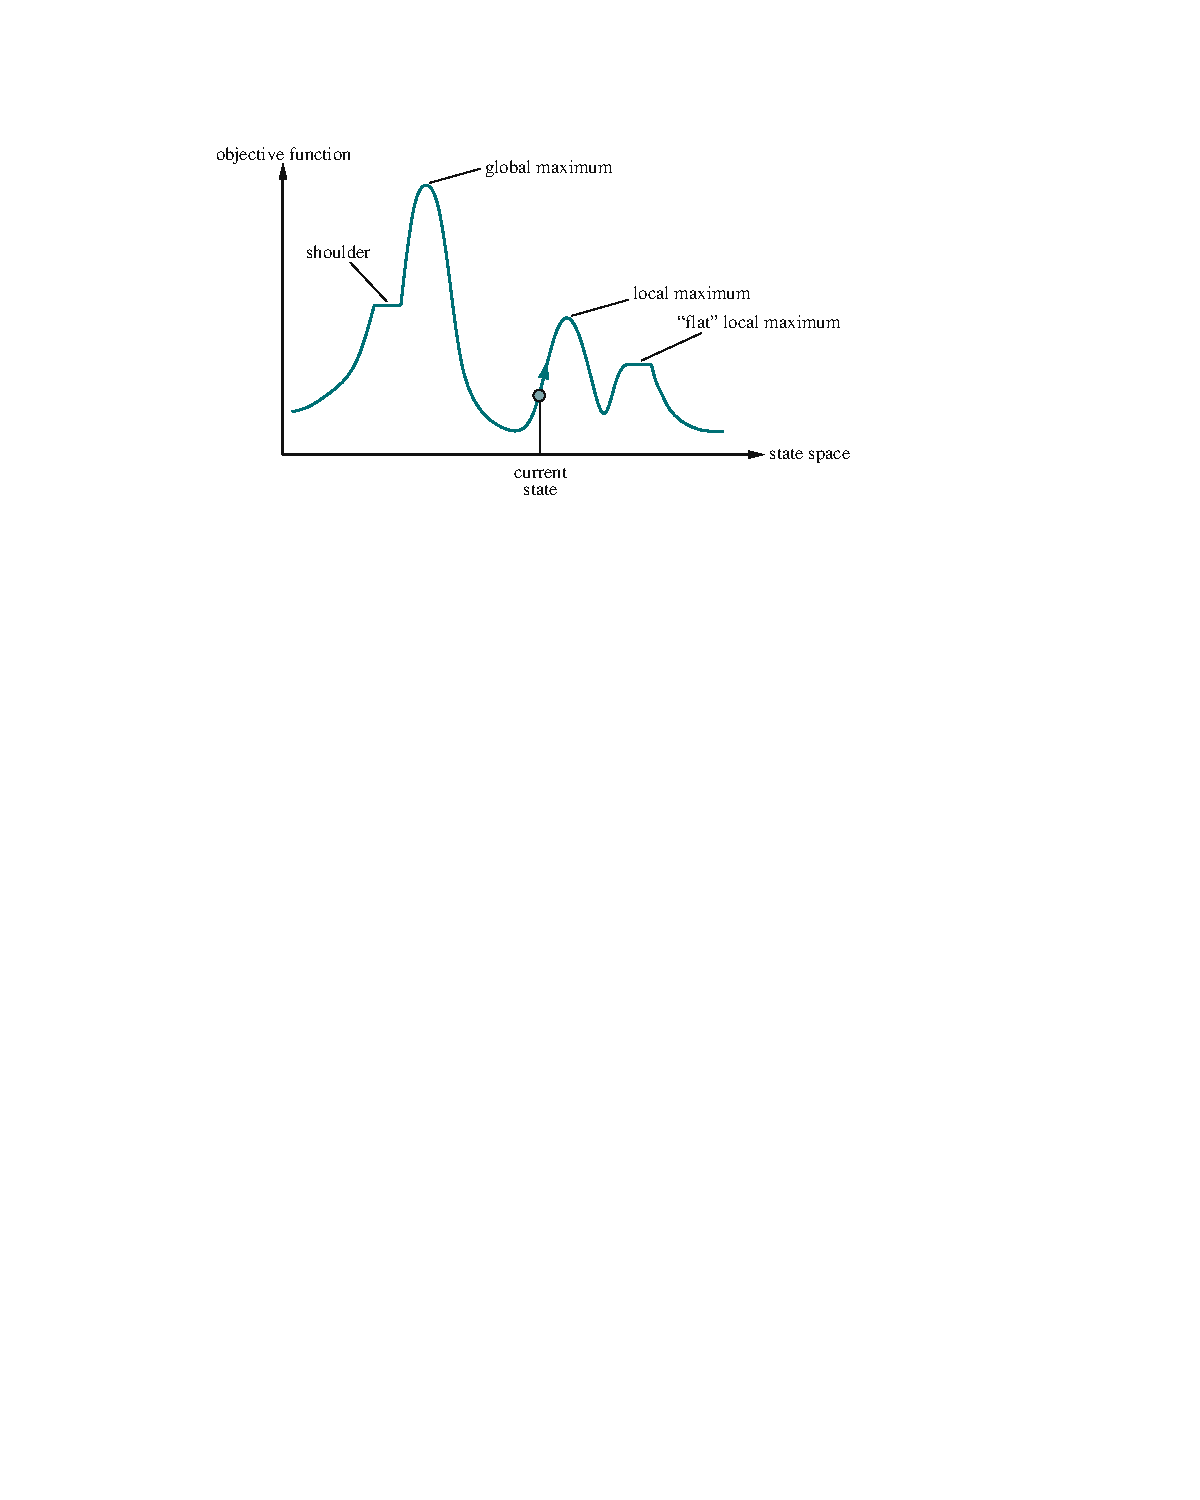
\includegraphics[alt={aima fig 04_01 state space landscape},width=0.75\linewidth]{aima-fig-04_01-state-space-landscape.pdf}
\section{Hill-Climbing Search}
\label{sec:orgff47282}


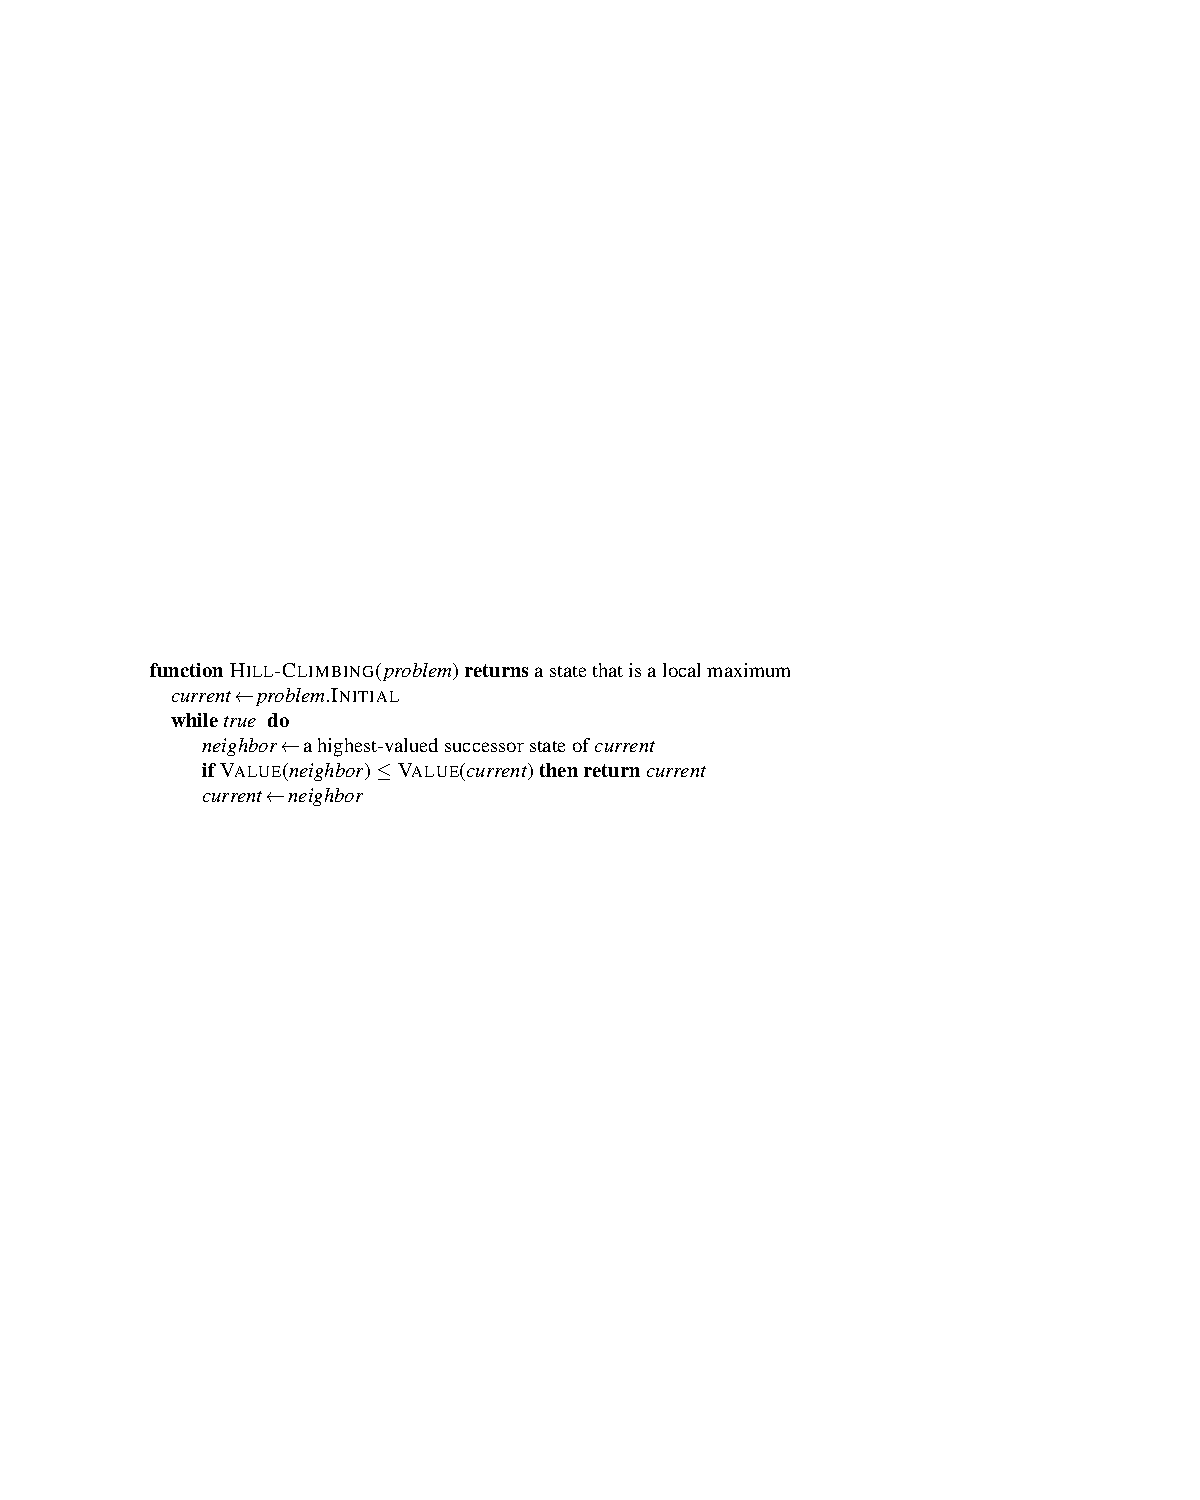
\includegraphics[alt={aima fig 04_02 hill climbing algorithm},width=0.75\linewidth]{aima-fig-04_02-hill-climbing-algorithm.pdf}


Also known as \textbf{greedy local search}.
\section{The 8 Queens Problem}
\label{sec:org750ca0d}

\textbf{Complete-state formulation}: each state has all components of a solution.

\begin{itemize}
\item 8 Queens state: row position for each of 8 columns, e.g., (a) below is ``
\end{itemize}


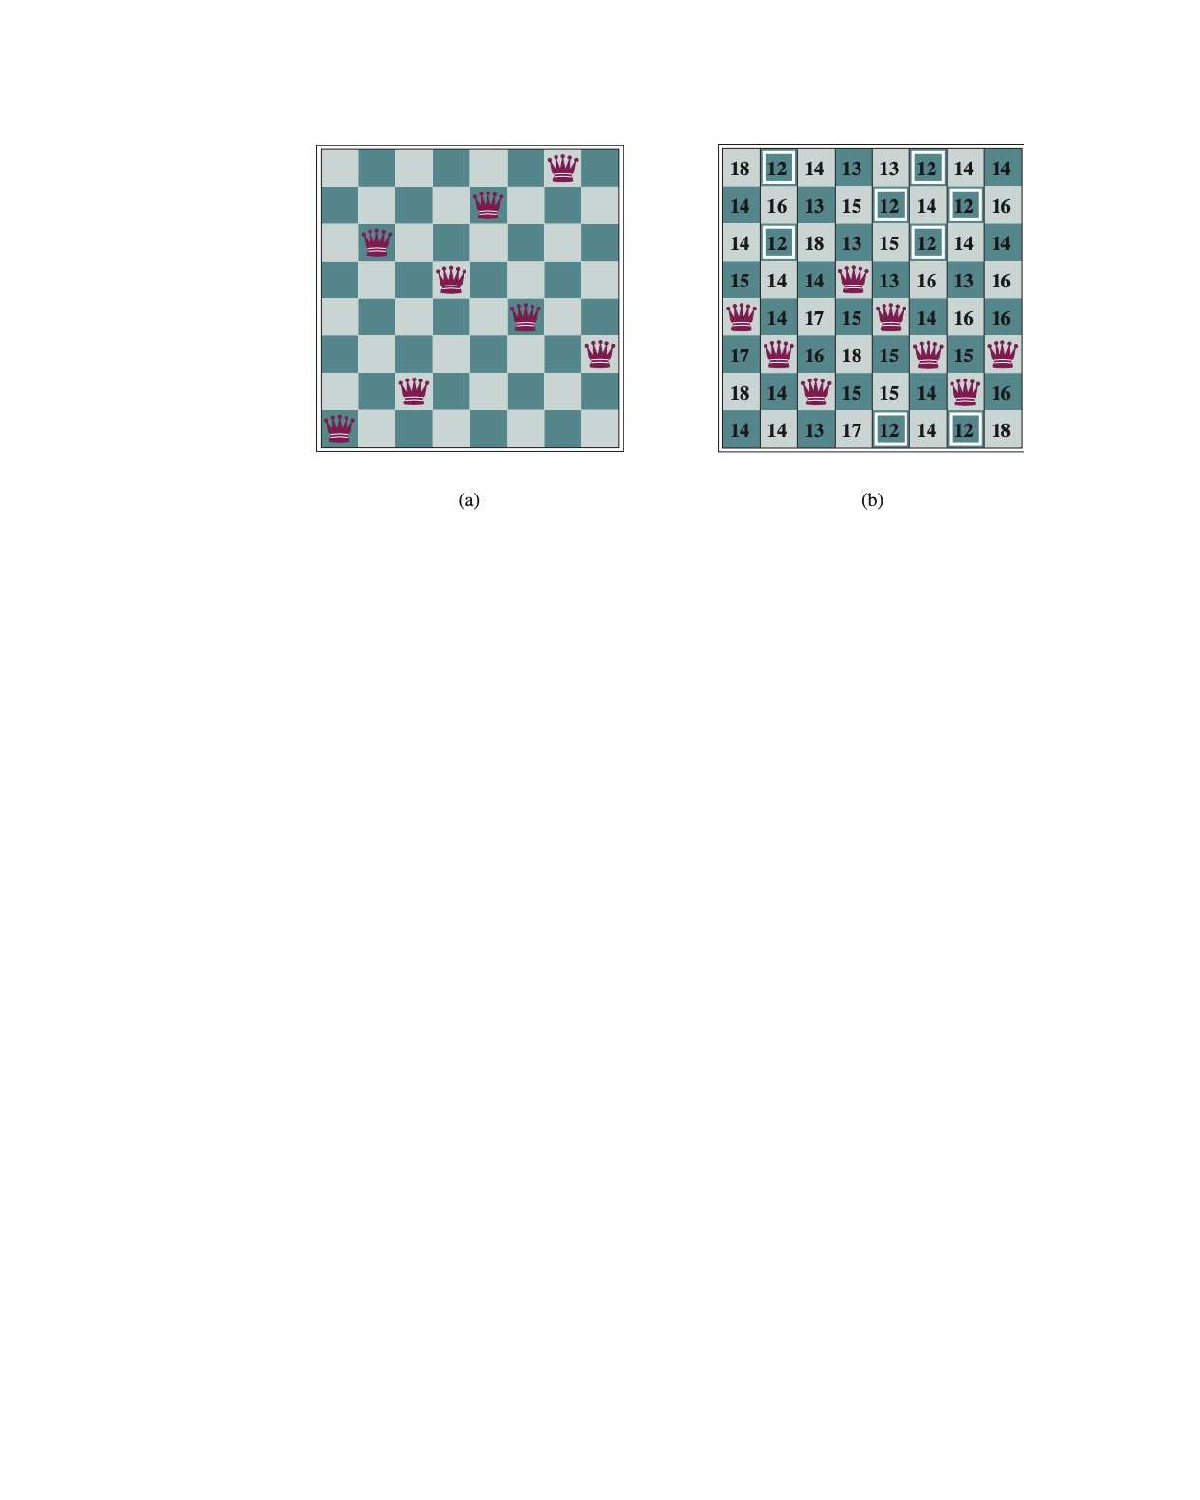
\includegraphics[alt={aima fig 04_03 8 queens},height=2.0in]{aima-fig-04_03-8-queens.pdf}


\begin{itemize}
\item Action: move a single queen to new row within column.  Each state has \(8 \cdot 7 = 56\) successor states.
\item Possible heuristic: number of pairs of attacking queens (even if blocked).  (b) above has \(h = 17\).

\begin{itemize}
\item Useful to remember: \(\binom{n}{k} = \frac{n!}{k!(n-k)!}\)
\end{itemize}
\end{itemize}
\section{Disadvantages of Hill-Climbing}
\label{sec:org426460c}



Susceptible to getting stuck in:

\begin{itemize}
\item local maxima
\item ridges -- sequences of local maxima
\item plateaus, e.g., flat local maxima or shoulders.
\end{itemize}

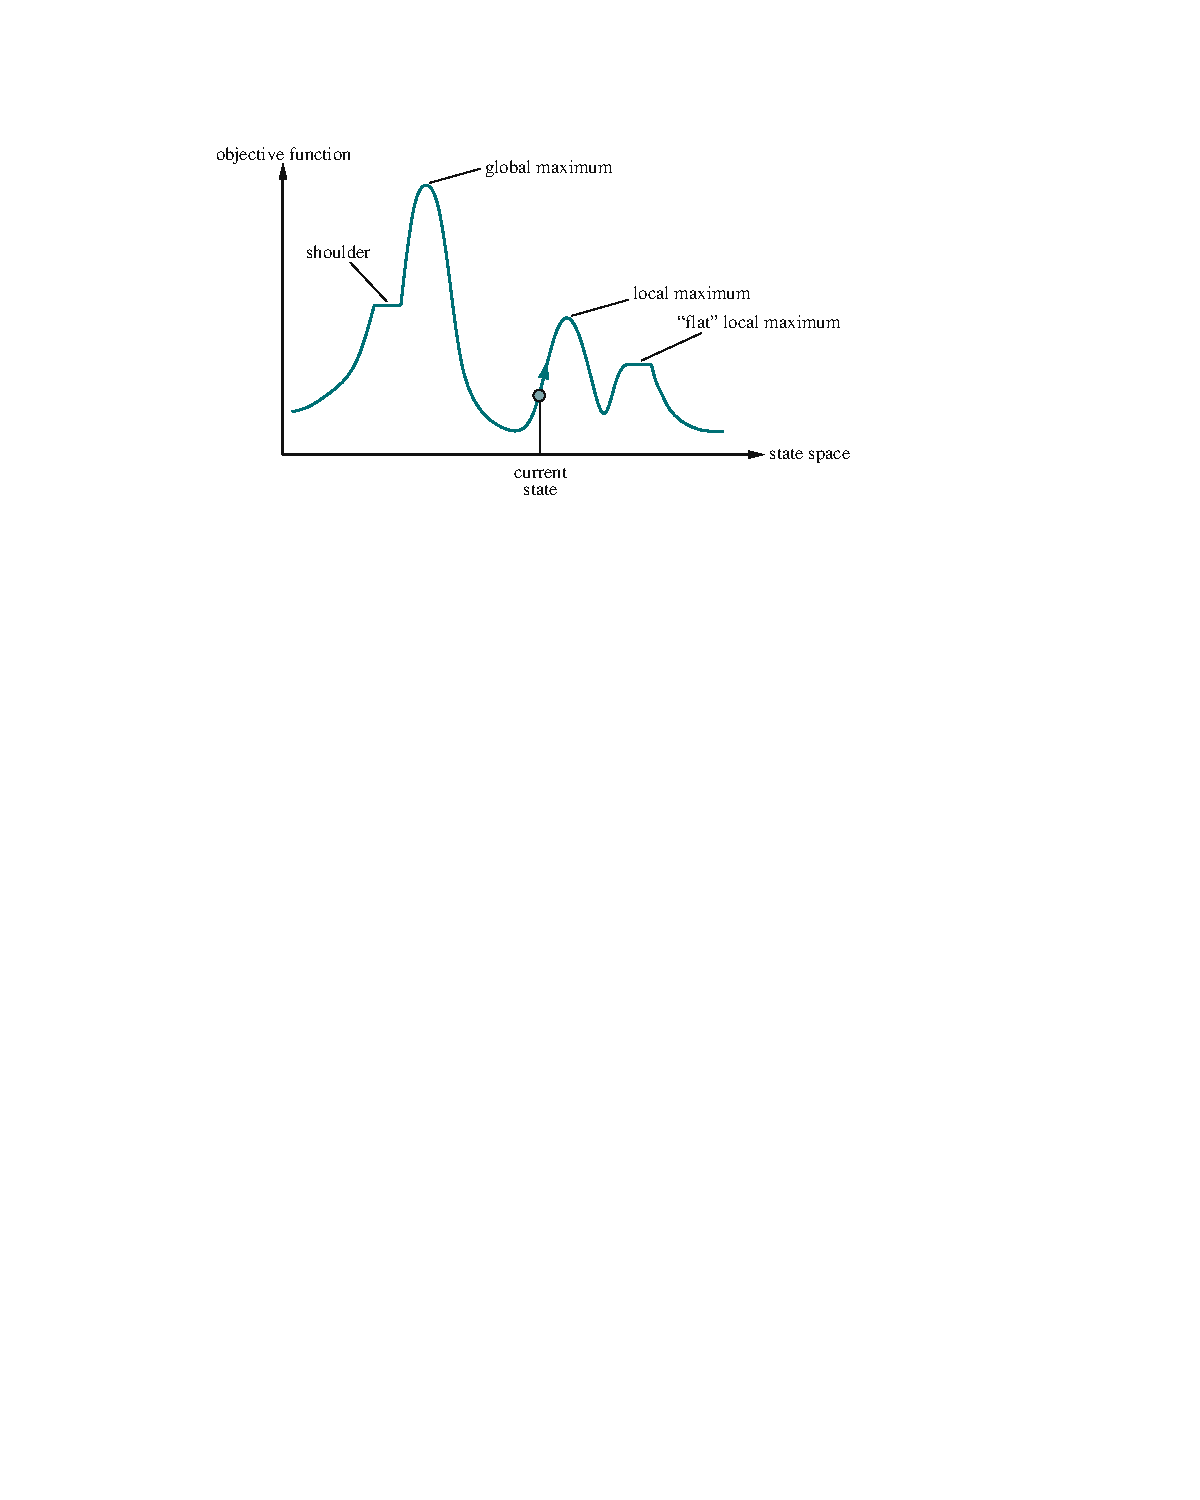
\includegraphics[alt={aima fig 04_01 state space landscape},height=1.6in]{aima-fig-04_01-state-space-landscape.pdf}

How to fix:

\begin{itemize}
\item Allow "sideways" moves
\item Stochastic hill climbing chooses randomly from uphill moves. Stochastic beam search does this with \(k\) states in parallel.
\item Random restart hill climbing restarts from multiple initial states.
\end{itemize}




Grid of states superimposed on ridge rising from left to right.


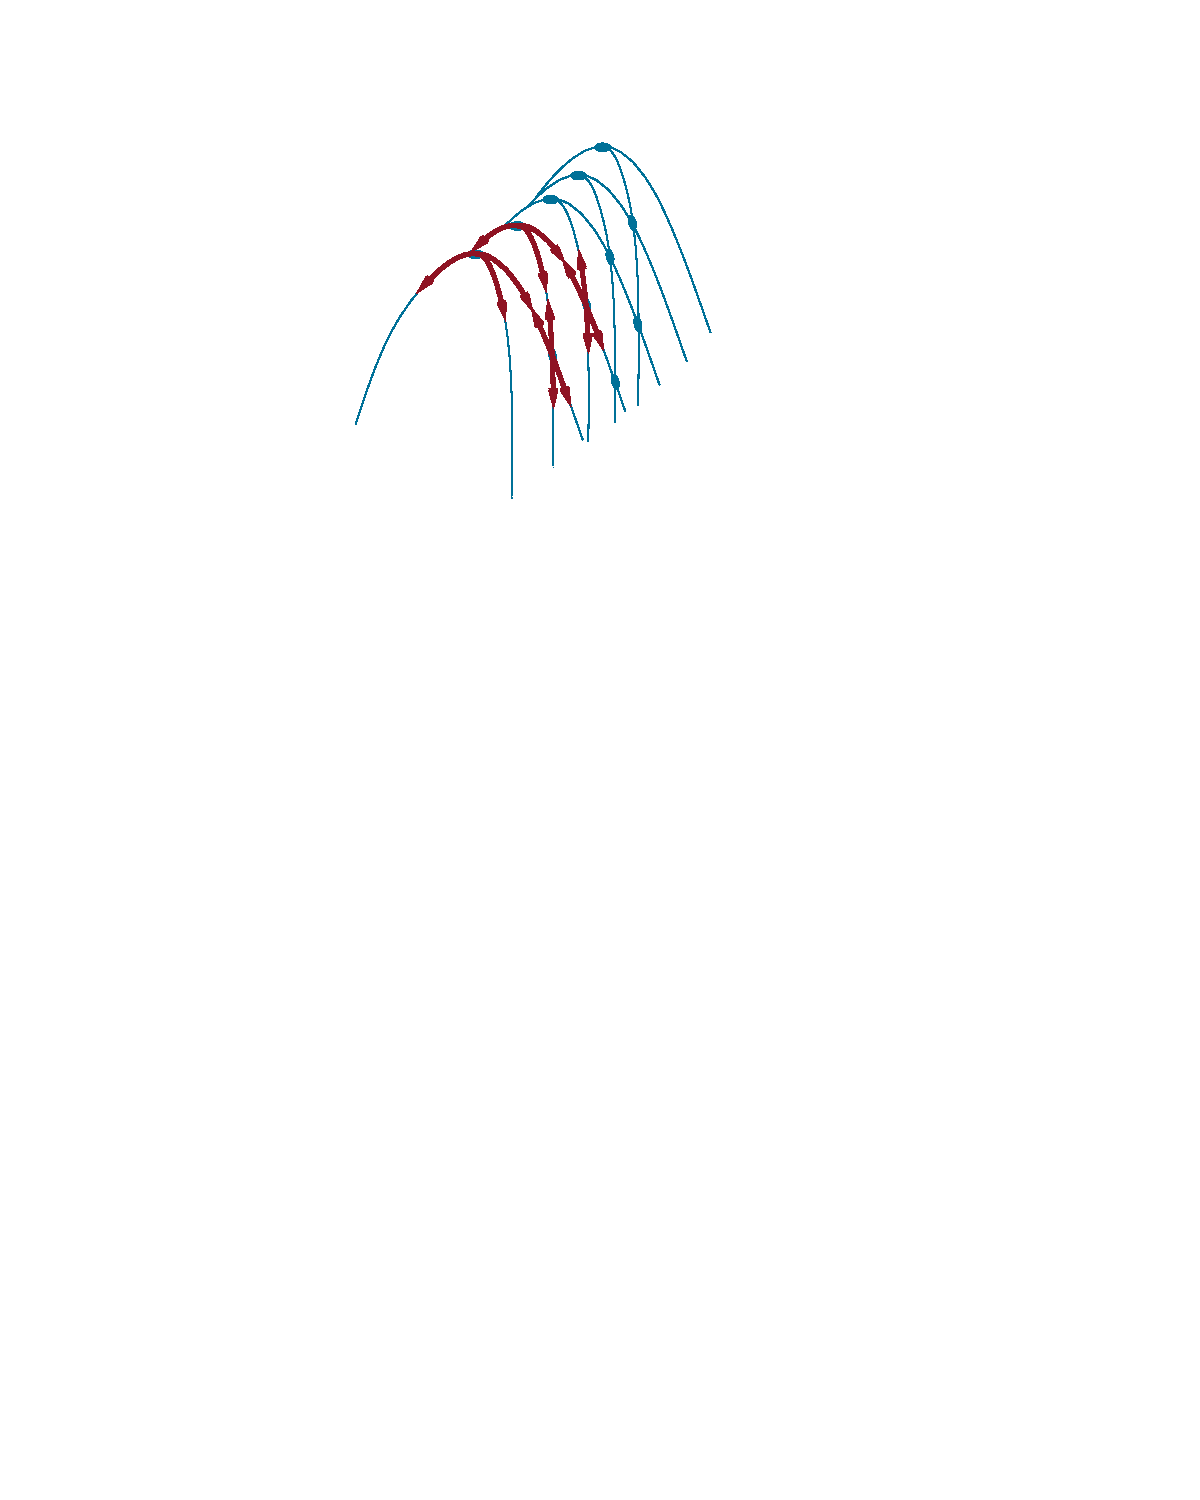
\includegraphics[alt={aima fig 04_04 ridges},width=0.75\linewidth]{aima-fig-04_04-ridges.pdf}
\section{Simulated Annealing}
\label{sec:org03f5aa1}


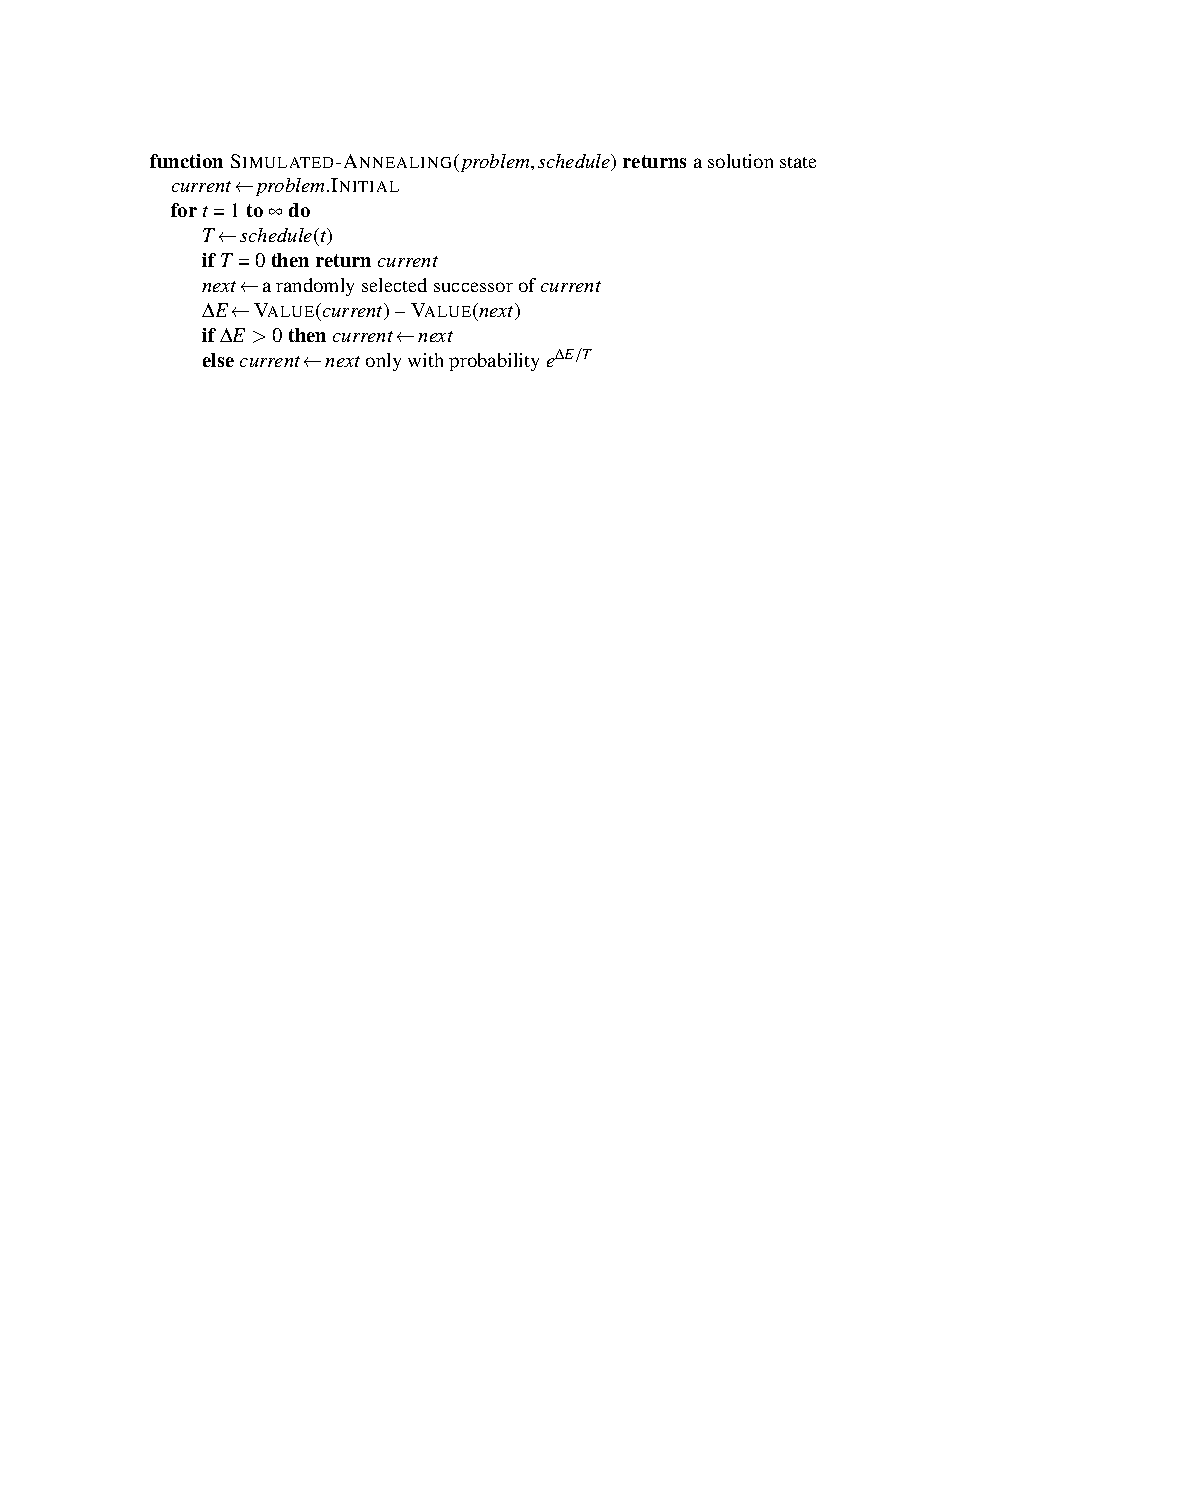
\includegraphics[alt={aima fig 04_05 simulated annealing algorithm},height=1.2in]{aima-fig-04_05-simulated-annealing-algorithm.pdf}


\begin{itemize}
\item Based on metallurgy -- gradually cool metal to reach low-energy crystalline state.
\item Intuition: think of gradient descent instead of gradient ascent -- multiple shallow valleys, one deepest valley.  Shake ball out of shallow valleys into deepest valley.
\item Similar to hill climbing, but picks a random move and

\begin{itemize}
\item accepts it if its better,
\item if not better, accept with probability < 1.
\end{itemize}

\item Probability of accepting a worse move depends on:

\begin{itemize}
\item how much worse the move is, \(\Delta E\), and
\item the current "temperature," \(T\).
\end{itemize}
\end{itemize}

If \(T\) decreases sufficiently slowly, then the Boltzman distribution, \(e^{\frac{\Delta E}{T}}\), ensures that all the probability is concentrated on the global maxima, so the algorithm finds a global maximum with probability approaching 1.
\section{Evolutionary (Genetic) Algorithms}
\label{sec:orgdb0cf76}

A kind of \textbf{local beam search}: tracking \(k\) states instead of just one.

Elements of genetic algorithms:

\begin{itemize}
\item Fitness function.
\item Population size.
\item Candidate representation:

\begin{itemize}
\item Typically a string (vector) over a finite alphabet.
\item \textbf{Evolution strategies}: sequence of real numbers.
\item \textbf{Genetic programming}: computer programs.
\end{itemize}

\item Mixing number, \(\rho\): number of "parents" from which to generate new candidates.  When \(\rho = 1\), stochastic beam search.
\item Selection process for choosing "parents."
\item Recombination procedure.
\item Mutation rate.
\item Composition of next generation.

\begin{itemize}
\item Elitism: choose top-scoring candidates.
\item Culling: eliminate bottom-scoring candidates.
\end{itemize}
\end{itemize}
\section{A Genetic Algorithm}
\label{sec:orgffc7b23}


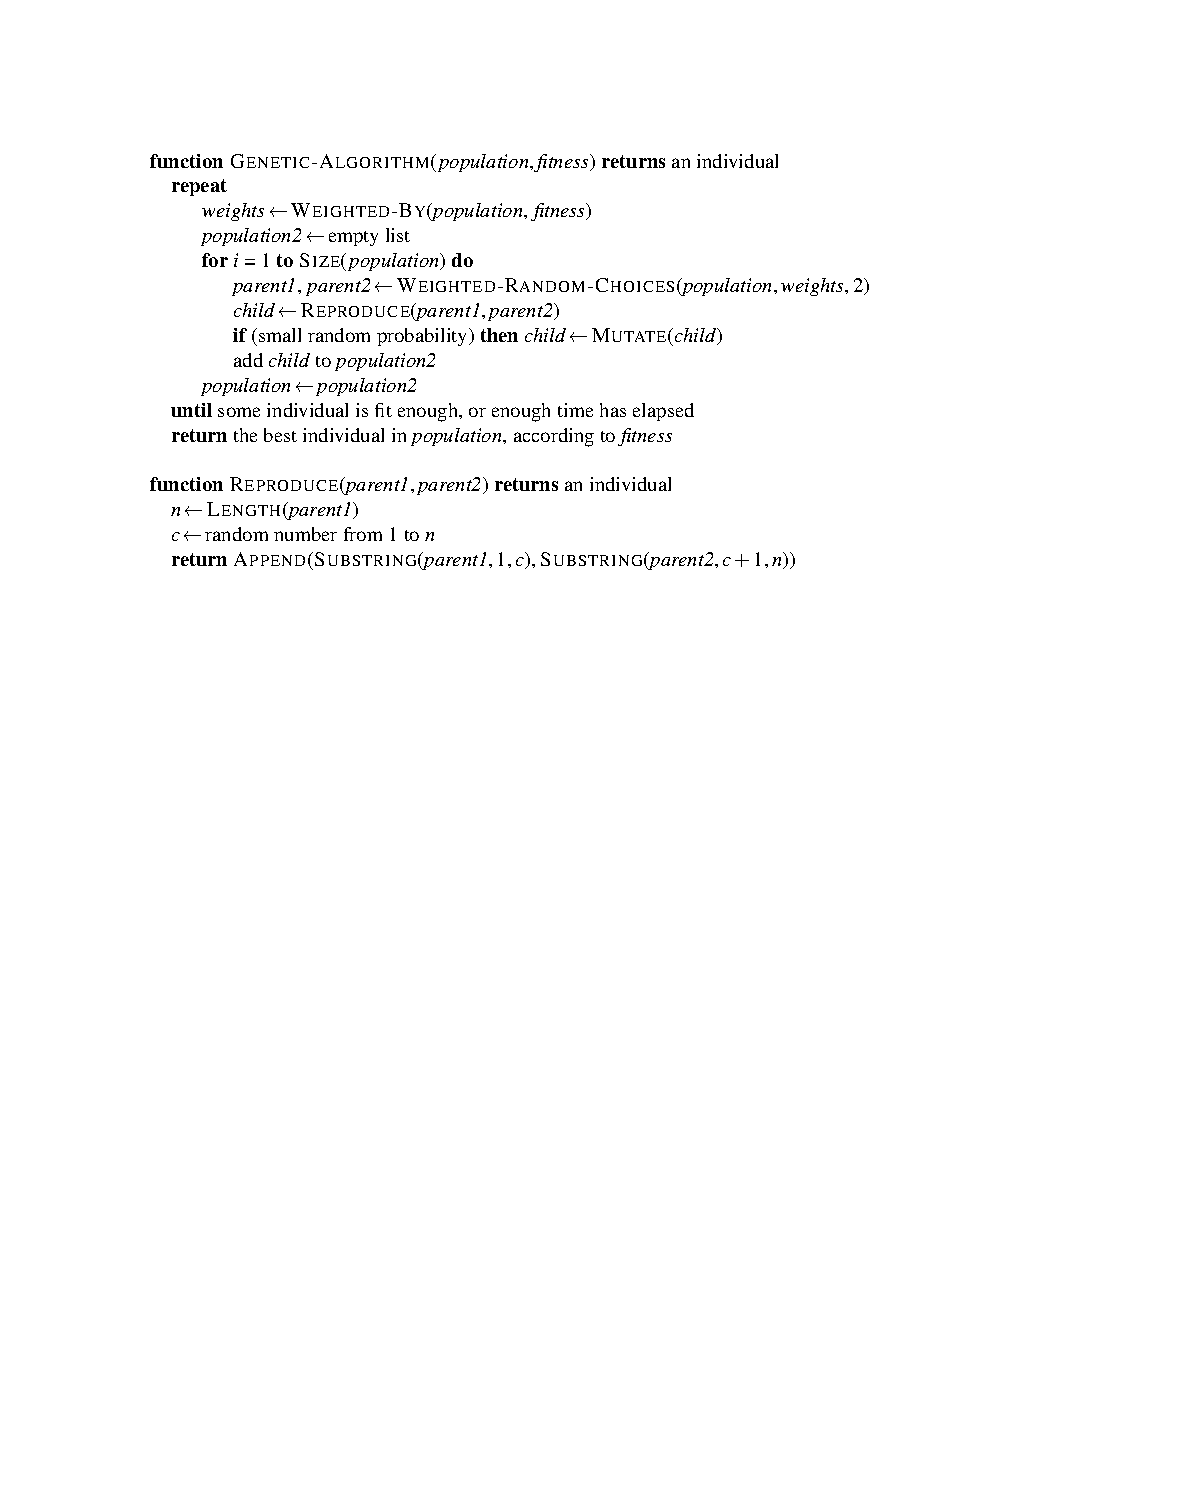
\includegraphics[alt={aima fig 04_08 genetic algorithm},width=0.75\linewidth]{aima-fig-04_08-genetic-algorithm.pdf}
\section{Genetic Algorithm on 8-Queens Problem}
\label{sec:org8d23d2a}


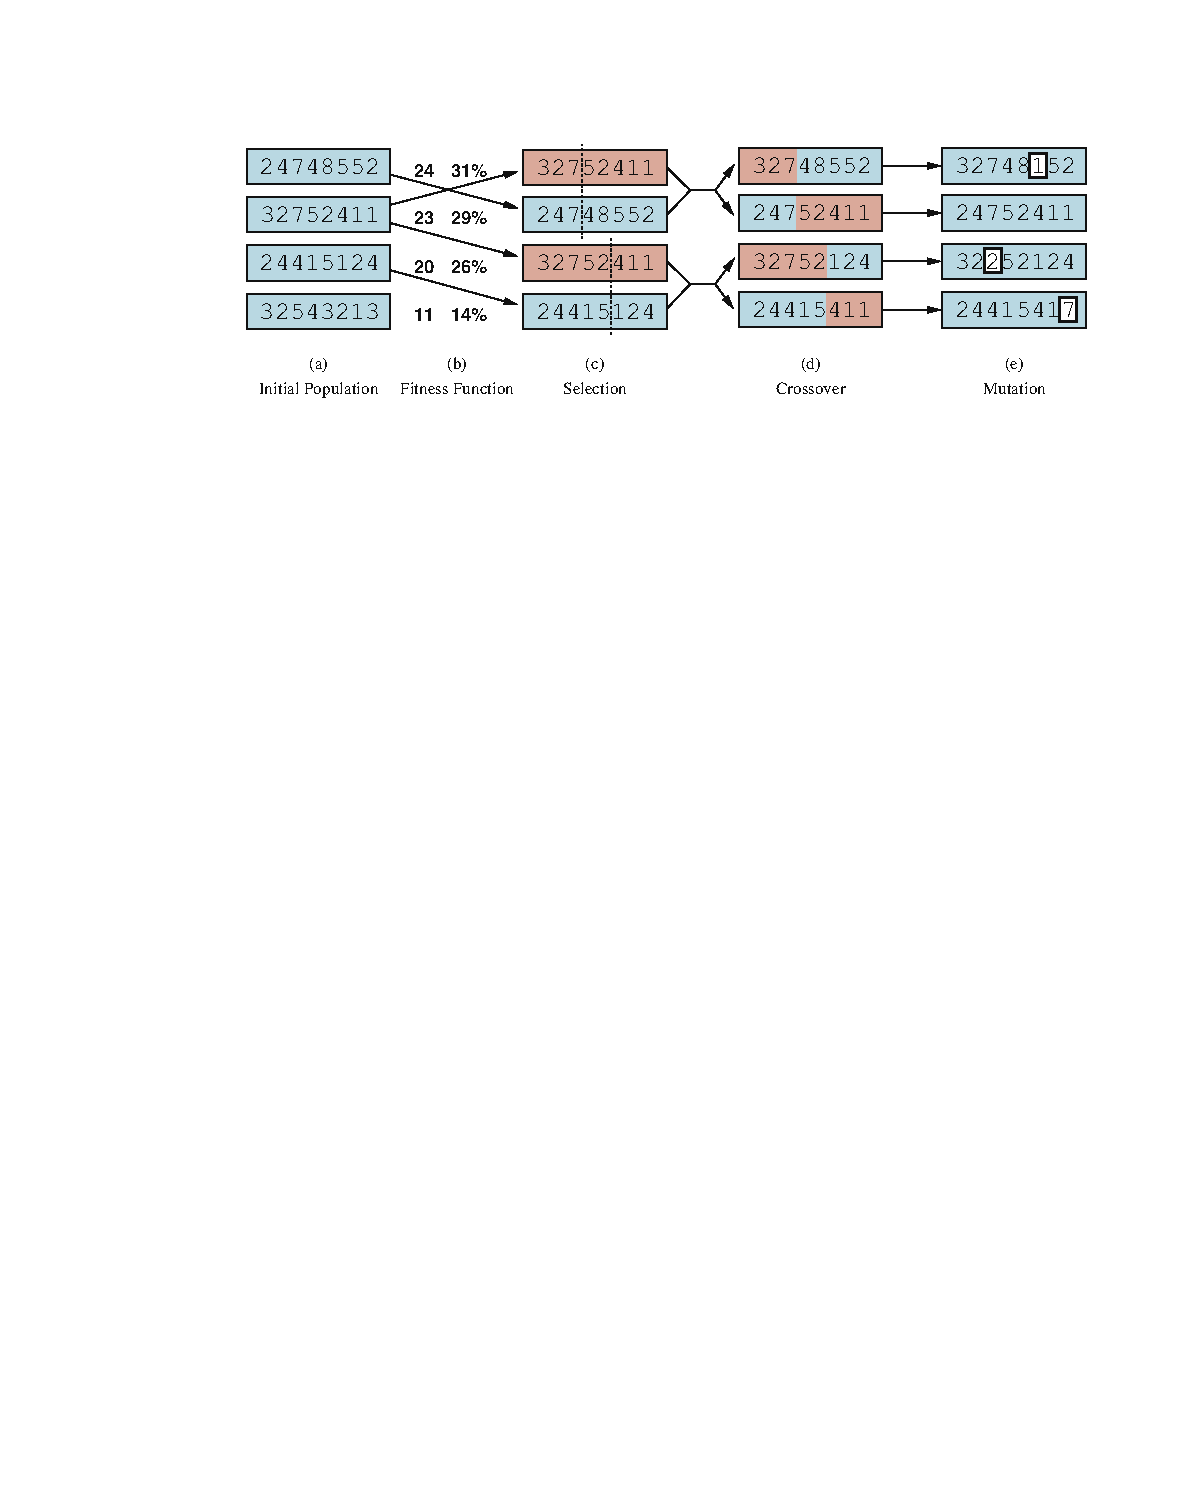
\includegraphics[alt={aima fig 04_06 genetic algorithm 8 queens illustration},width=0.75\linewidth]{aima-fig-04_06-genetic-algorithm-8-queens-illustration.pdf}


\begin{enumerate}
\item Population is generated in (a).
\item Fitness function is applied to population, which is then ranked by fitness score.
\item Highest-scoring candidates are selected for reproduction in (c).
\item Crossover operation is applied to candidates in (c) to produce "children" in (d).
\item In (e) "offspring" are randomly chosen for mutation.  For each chosen candidate, a "gene" is randomly chosen, then that gene is assigned a random "mutated" value.
\end{enumerate}
\section{Crossover in the 8-queens Problem}
\label{sec:org5517327}

Here is a pictorial illustration of the crossover operation in the 8-queens problem:


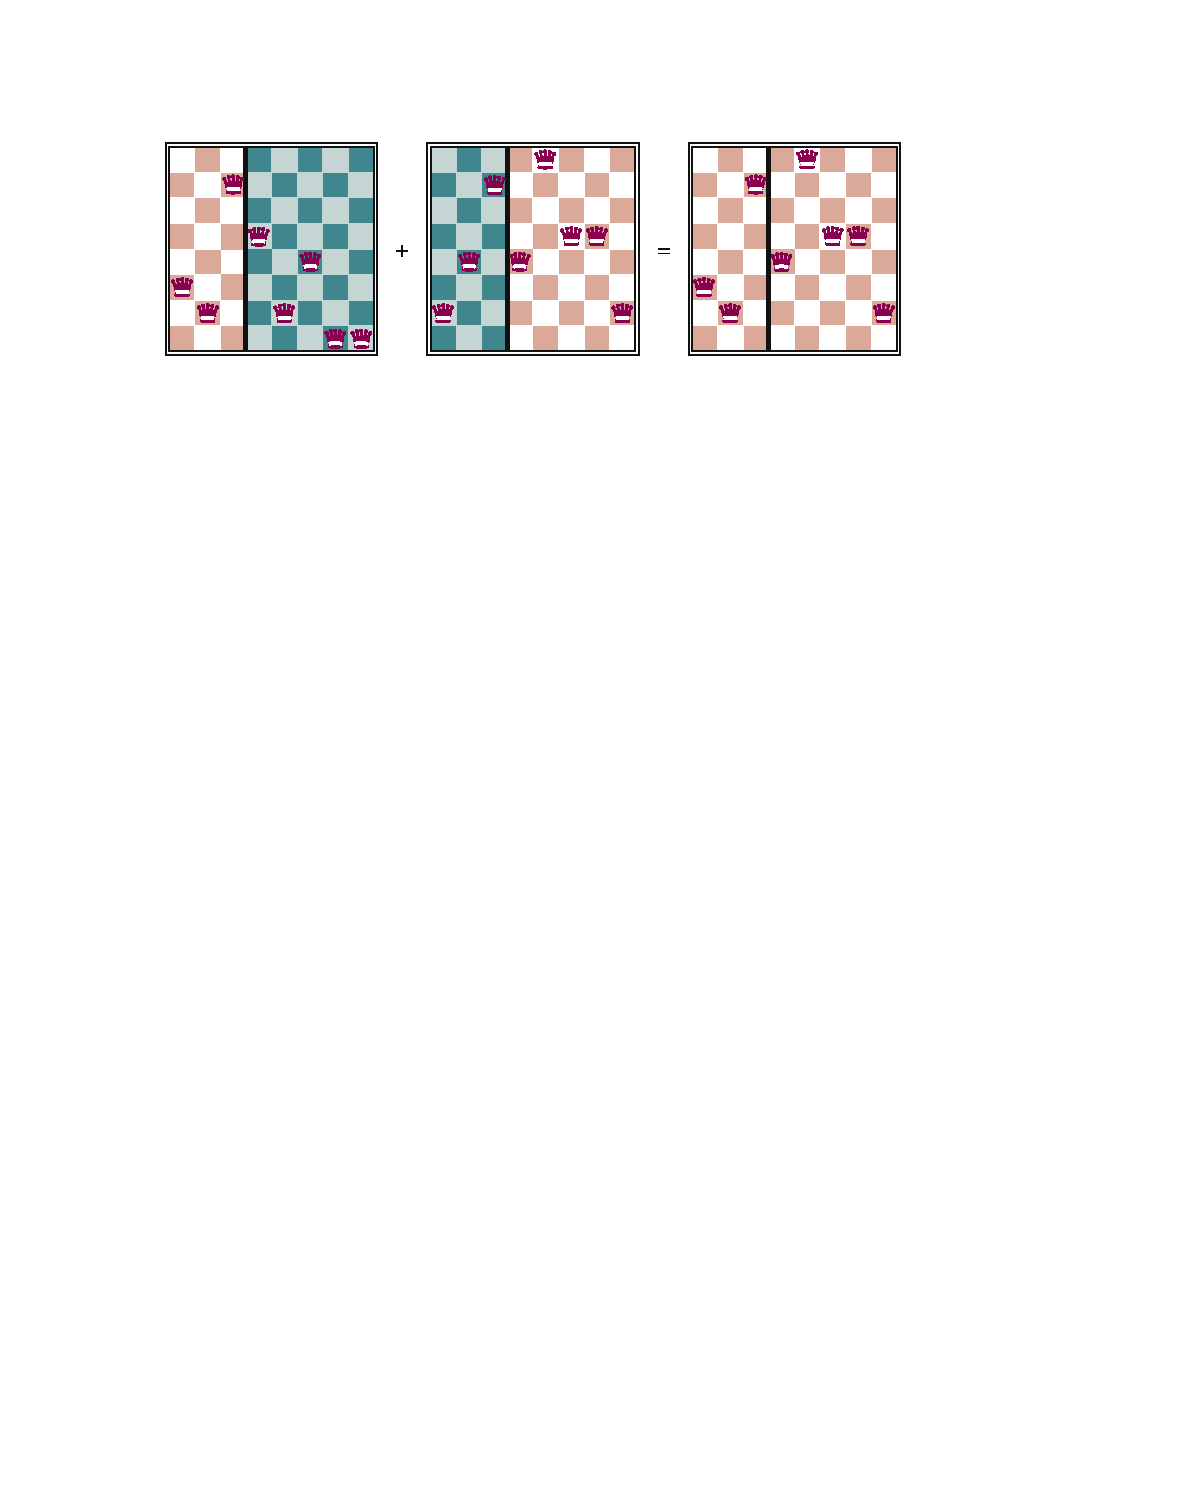
\includegraphics[alt={aima fig 04_07 8 queens crossover diagrams},width=0.75\linewidth]{aima-fig-04_07-8-queens-crossover-diagrams.pdf}


Is the random crossover operation depicted here meaningful for the 8-queens problem?
\section{Genetic Algorithms and Biological Evolution}
\label{sec:orgf088406}

Genetic algorithms borrow the language of biological evolution for marketing purposes, but are far more simplistic than biological evolution.  My takes:

\begin{itemize}
\item Genetic algorithms are just stochastic beam search with "sexual" successor generation and "mutation."
\item If there is no meaningful crossover operation, genetic algorithms are just random walks in the state space graph.
\end{itemize}

There is an interesting connection between biological evolution and AI, in particular learning.

\begin{itemize}
\item Learning is adaptation. With experience an agent adapts to a task, getting better at the task.
\item Biological evolution can be seen as a learning process whereby specieses "learn" to perform better in their environments.
\item The Baldwin effect: immutable traits vs. online learning ability.

\begin{itemize}
\item Plasticity, or the ability to learn, allows a species to adapt to an environment for which it is ill-suited.  E.g., building shelters, fire, etc. in cold regions.
\item Things that are harder, or impossible, to learn online must be encoded in the genome.  E.g., the way our body uses the air it breathes or the sun.
\end{itemize}
\end{itemize}
\section{Continuous State Spaces -- Airports In Romania}
\label{sec:org032cd9b}






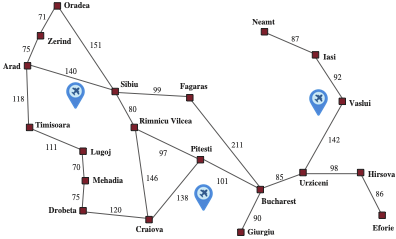
\includegraphics[alt={aima romania airports},height=3.2in]{aima-romania-airports.png}





If each airport \(\bm{x}_i\) is at location \((x_i, y_i)\) and the set of cities closest to airport \(\bm{x}_i\) is \(C_i\), then

\begin{equation*}
f(\bm{x}) = f(x_1, y_1, x_2, y_2, x_3, y_3)
\end{equation*}

and we want to minimize

\begin{equation*}
f(\bm{x}) = \sum_{i=1}^3 \sum_{c \in C_i} (x_i - x_c)^2 + (y_i - y_c)^2
\end{equation*}

For a globally optimal solution, if the airports move "too much," the sets \(C_i\) change.  How to deal with that?
\section{Local Gradient Descent}
\label{sec:org23397ab}

The gradient of

\begin{equation*}
f(\bm{x}) = \sum_{i=1}^3 \sum_{c \in C_i} (x_i - x_c)^2 + (y_i - y_c)^2
\end{equation*}

is

\begin{equation*}
\nabla f = \left( \frac{\partial f}{\partial x_1},
                  \frac{\partial f}{\partial y_1},
                  \frac{\partial f}{\partial x_2},
                  \frac{\partial f}{\partial y_2},
                  \frac{\partial f}{\partial x_3},
                  \frac{\partial f}{\partial y_3} \right)
\end{equation*}

But that would only work for one airport.  We can decompose it into three local problems:




\begin{equation*}
\frac{\partial f}{\partial x_1} = 2 \sum_{c \in C_1} (x_1 - x_c)
\end{equation*}
\begin{equation*}
\frac{\partial f}{\partial y_1} = 2 \sum_{c \in C_1} (y_1 - y_c)
\end{equation*}




\begin{equation*}
\frac{\partial f}{\partial x_2} = 2 \sum_{c \in C_2} (x_2 - x_c)
\end{equation*}
\begin{equation*}
\frac{\partial f}{\partial y_2} = 2 \sum_{c \in C_2} (y_2 - y_c)
\end{equation*}




\begin{equation*}
\frac{\partial f}{\partial x_3} = 2 \sum_{c \in C_3} (x_3 - x_c)
\end{equation*}
\begin{equation*}
\frac{\partial f}{\partial y_3} = 2 \sum_{c \in C_3} (y_3 - y_c)
\end{equation*}
\section{Gradient Descent in Action}
\label{sec:org604da93}




Given our 3 gradient expressions, we can use the update rule:

\begin{equation*}
\bm{x} \leftarrow \bm{x} + \alpha \nabla f(\bm{x})
\end{equation*}

where \(\alpha\) is a \textbf{step size}, or learning rate.

\begin{itemize}
\item What if \(\alpha\) is "too big?"

\item What if \(\alpha\) is "too small?"
\end{itemize}





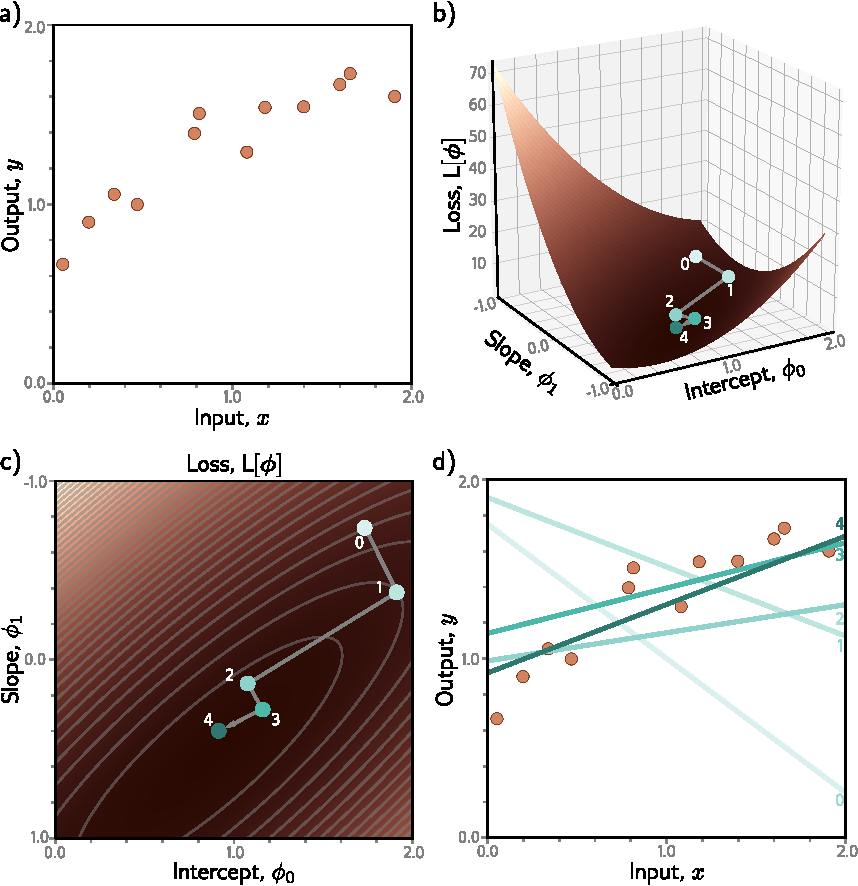
\includegraphics[alt={../../deep learning/slides/TrainLRMin},height=3.2in]{../../deep-learning/slides/TrainLRMin.pdf}





{[}\textsuperscript{UDLBook}]: \url{https://udlbook.github.io/udlbook/}
\section{Continuous State Spaces and Convexity}
\label{sec:org422af2e}

A convex set is a set of points in which a line between any two points lies within the set.  A convex function is a function for which the points above the function form a convex set.


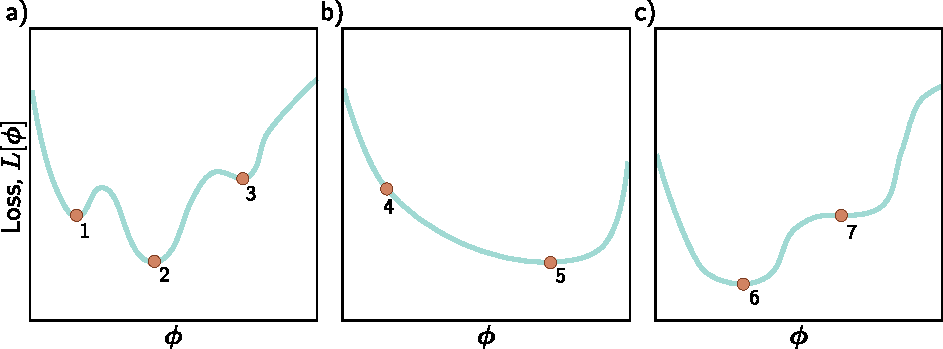
\includegraphics[alt={../../deep learning/slides/TrainConvexProb},width=0.75\linewidth]{../../deep-learning/slides/TrainConvexProb.pdf}


There are mathematical properties of continuous spaces that rule out local minima.  Take my deep learning class to learn about them!

{[}\textsuperscript{UDLBook}]: \url{https://udlbook.github.io/udlbook/}
\section{Constrained Optimization via Linear Programming}
\label{sec:org2af639b}




\begin{align*}
\text{maximize }    3x_1 + 2x_2  \\
\text{subject to }  -x_1 + 3x_2 &\le  12 \\
                    x_1 + x_2   &\le  8 \\
                    2x_1 - x_2  &\le  10 \\
                    x_1, x_2    &\ge  0
\end{align*}





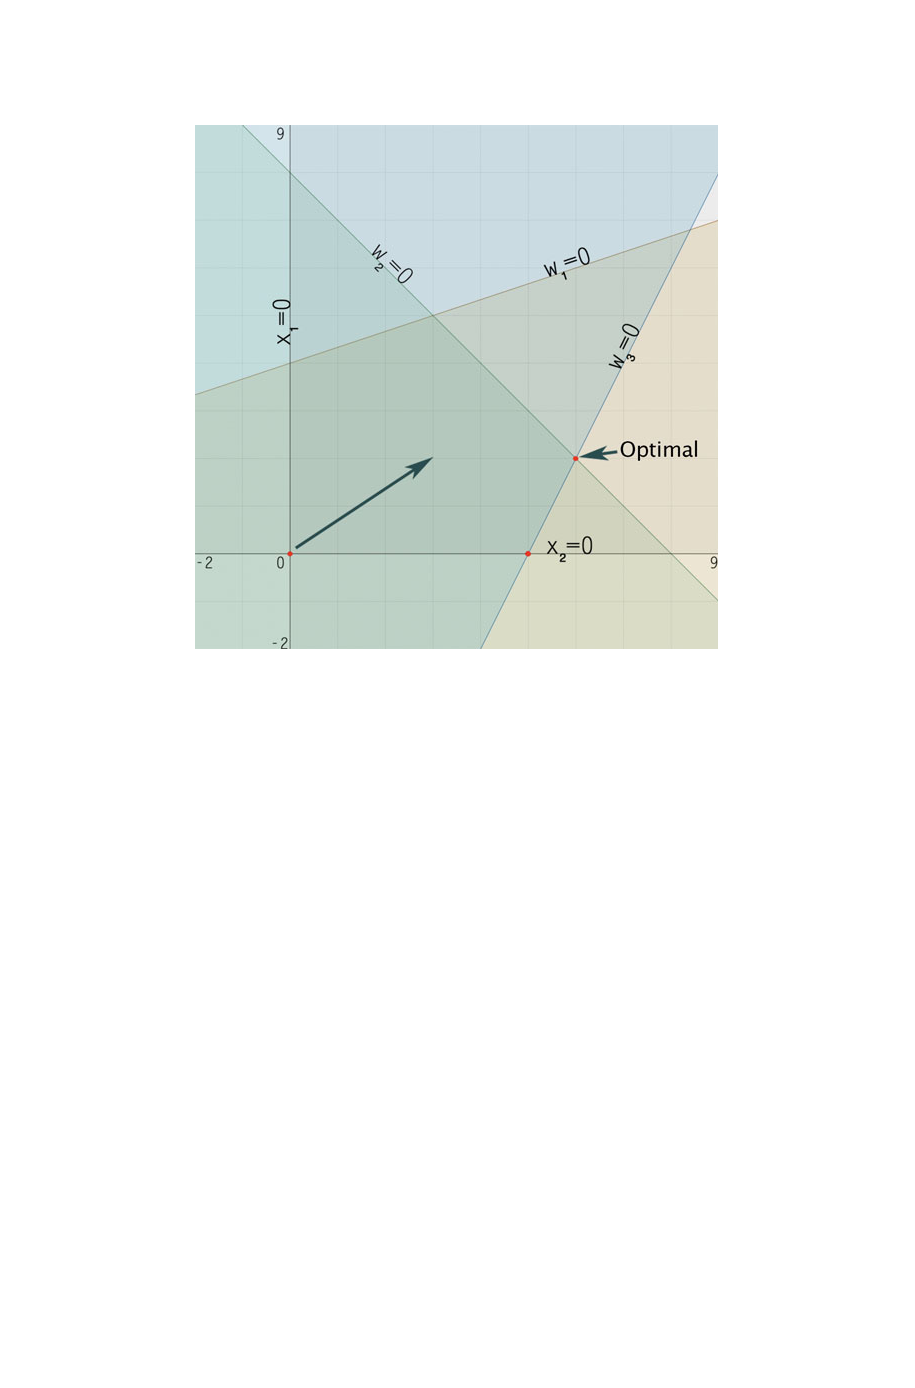
\includegraphics[alt={lp fig 02_01 half planes},height=2.8in]{lp-fig-02_01-half-planes.pdf}





{[}\textsuperscript{LPBook}]: \url{https://vanderbei.princeton.edu/LPbook/}
\end{document}
